\subsection{Ejercicio 17}
\graphicspath{ {img/17} }

\subsubsection{Circuito TOR}

El funcionamiento de TOR es crear una red con muchas capas, como si de una cebolla se tratara. El tráfico, en lugar de ir directamente del navegador al servidor de la web a la que el usuario se está intentando conectar pasa por una serie de servidores, los \textit{TOR Relays}. Podemos ver información sobre el circuito seleccionado en la barra de direcciones, como se muestra en la imagen:

\begin{figure}[H]
    \centering
    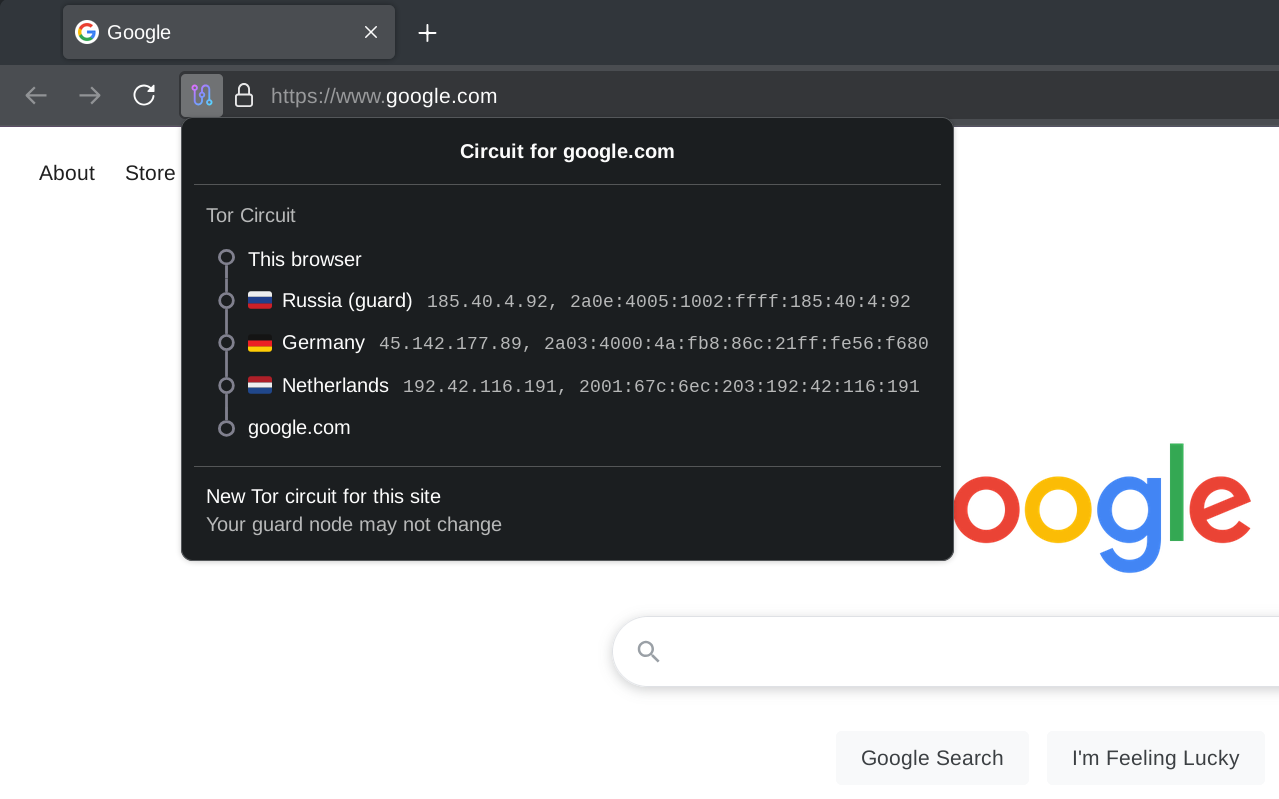
\includegraphics[width=\textwidth]{tor-google-circuit.png}
    \caption{Circuito con TOR}
\end{figure}

El circuito consta de tres nodos y se pueden cambiar, aunque el primer nodo, el nodo "guardia" no cambiará. Como el tráfico siempre pasa por este nodo durante una misma sesión, independientemente del sitio al que nos conectemos, desde el punto de vista de la operadora, siempre estamos accediendo al mismo sitio.

\subsubsection{Contenido en TOR}

Al conectarnos a través de TOR a \url{google.com} sí que vemos una diferencia con respecto a hacerlo con otro navegador, como Firefox, y es que en lugar de mostrarnos la versión del sitio web para españa, nos muestra la versión del Reino Unido, a pesar de que el nodo de salida de esta sesión está en Países Bajos y es desde ahí desde donde se conectaría a Google.

\begin{figure}[H]
    \centering
    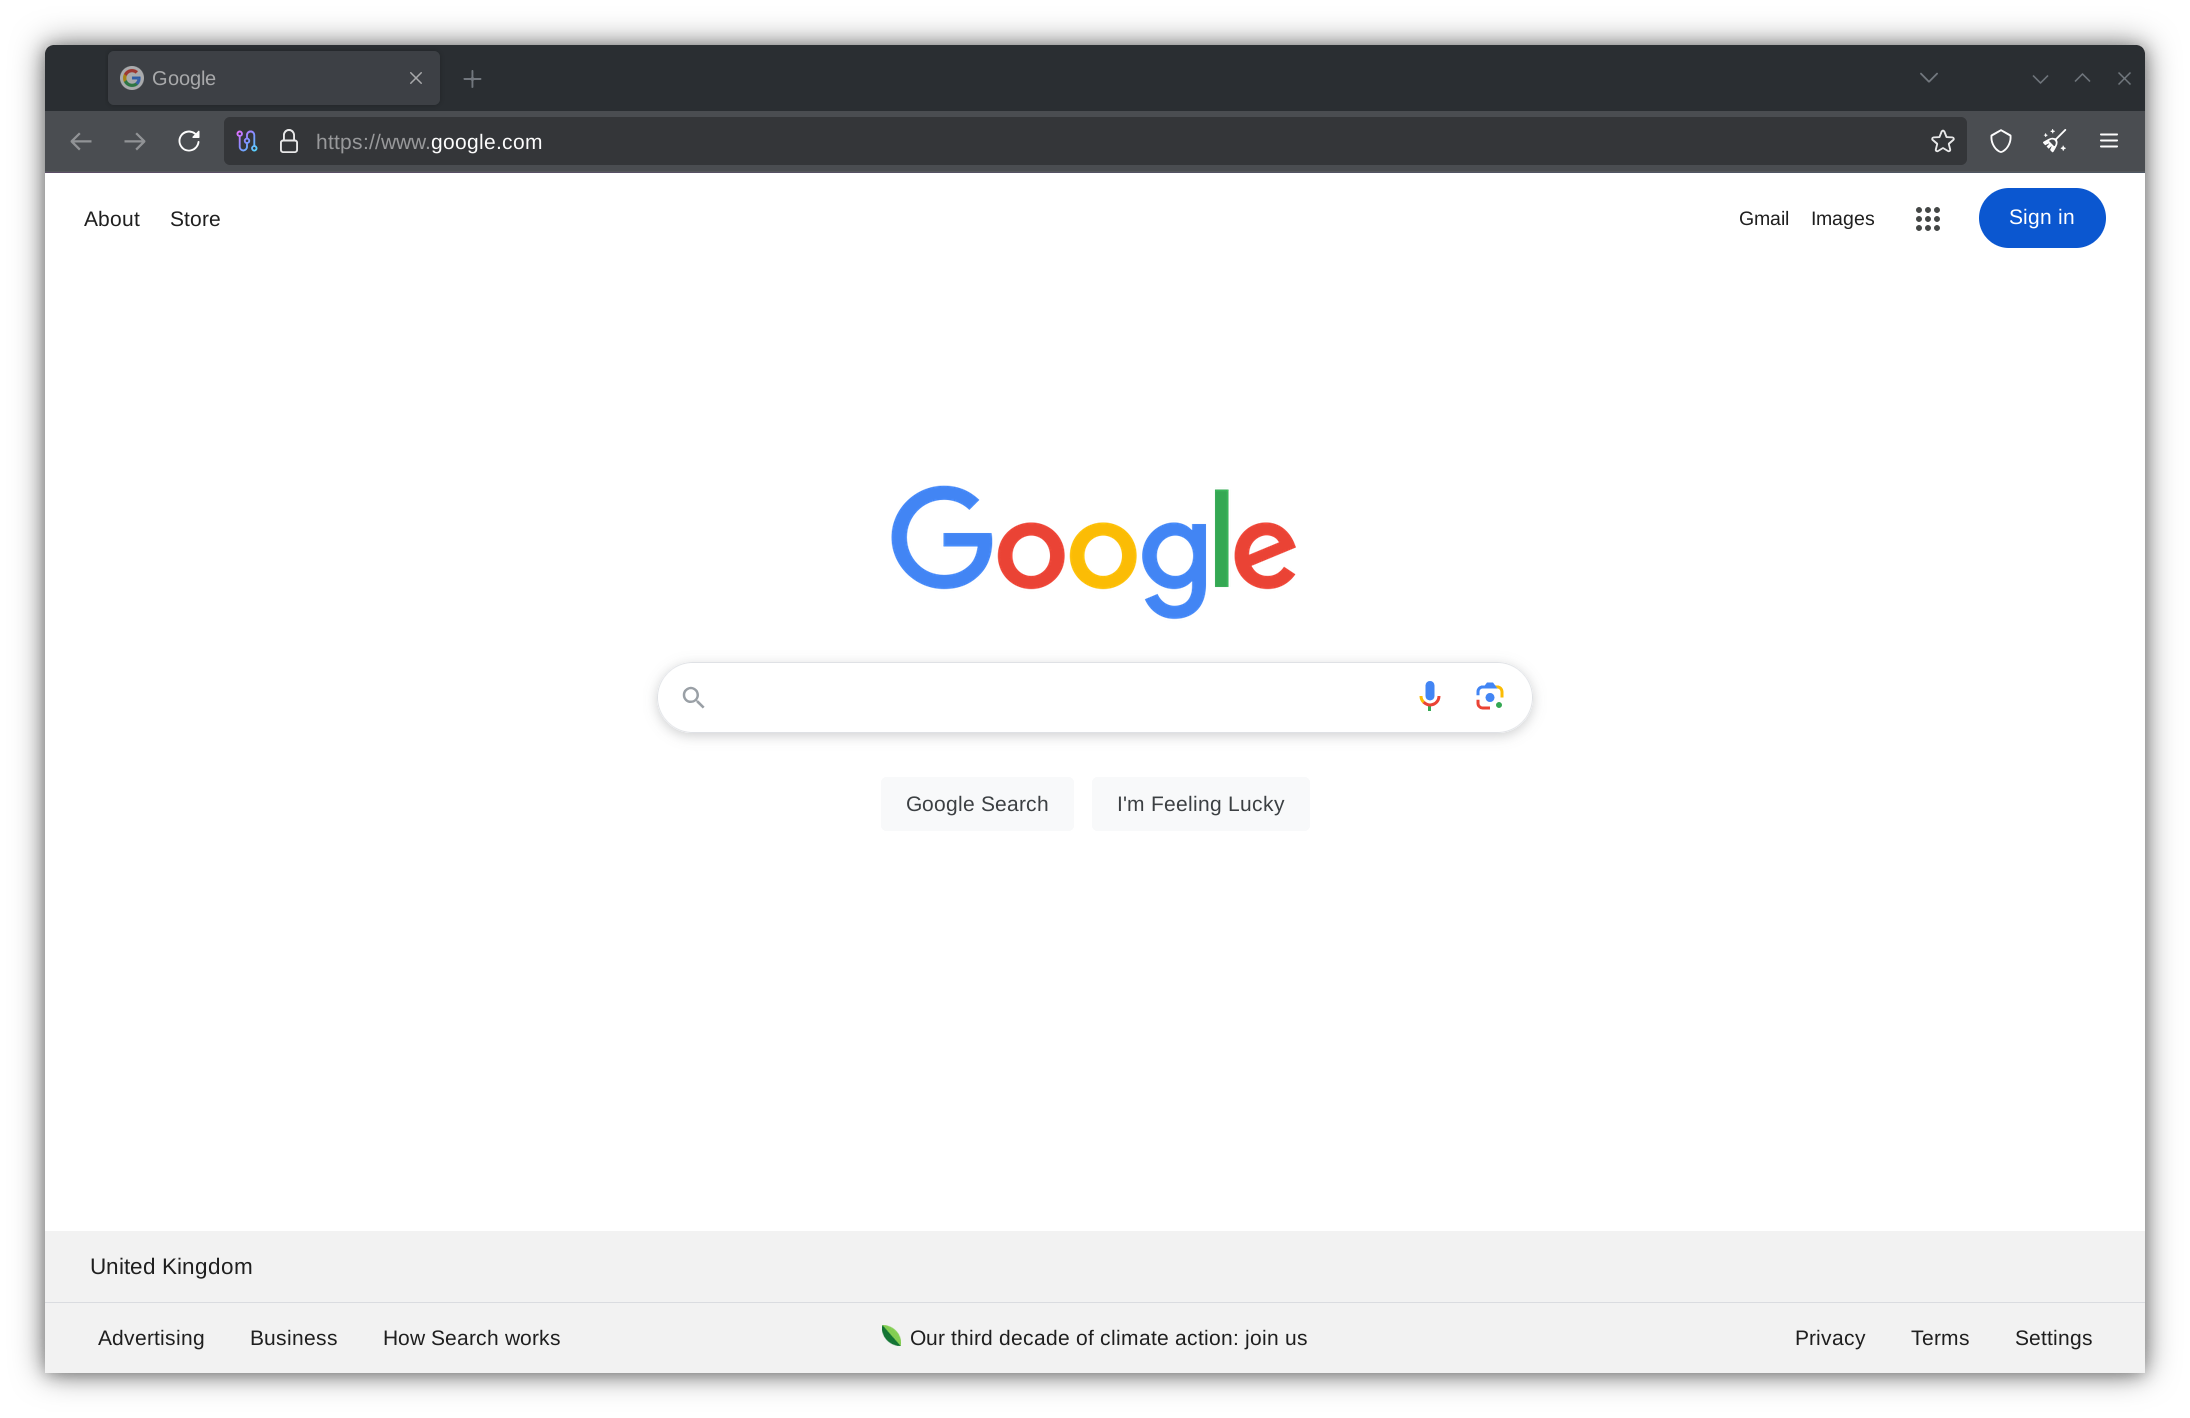
\includegraphics[width=\textwidth]{tor-google.png}
    \caption{\url{google.com} a través de TOR}
\end{figure}

\subsubsection{Cabecera HTTP \texttt{Onion-Location}}

La cabecera HTTP \texttt{Onion-Location} le indica a los usuarios del navegador TOR que el sitio al que están accediendo a través de HTTP, tiene una versión en la red de TOR utilizando el protocolo \texttt{onion}, y cual es su dirección ahí. El sitio web de Proton tiene esta cabecera y por eso en la barra de direcciones vemos un botón que indica que la versión \texttt{.onion} del sitio web está disponible.

\begin{figure}[H]
    \centering
    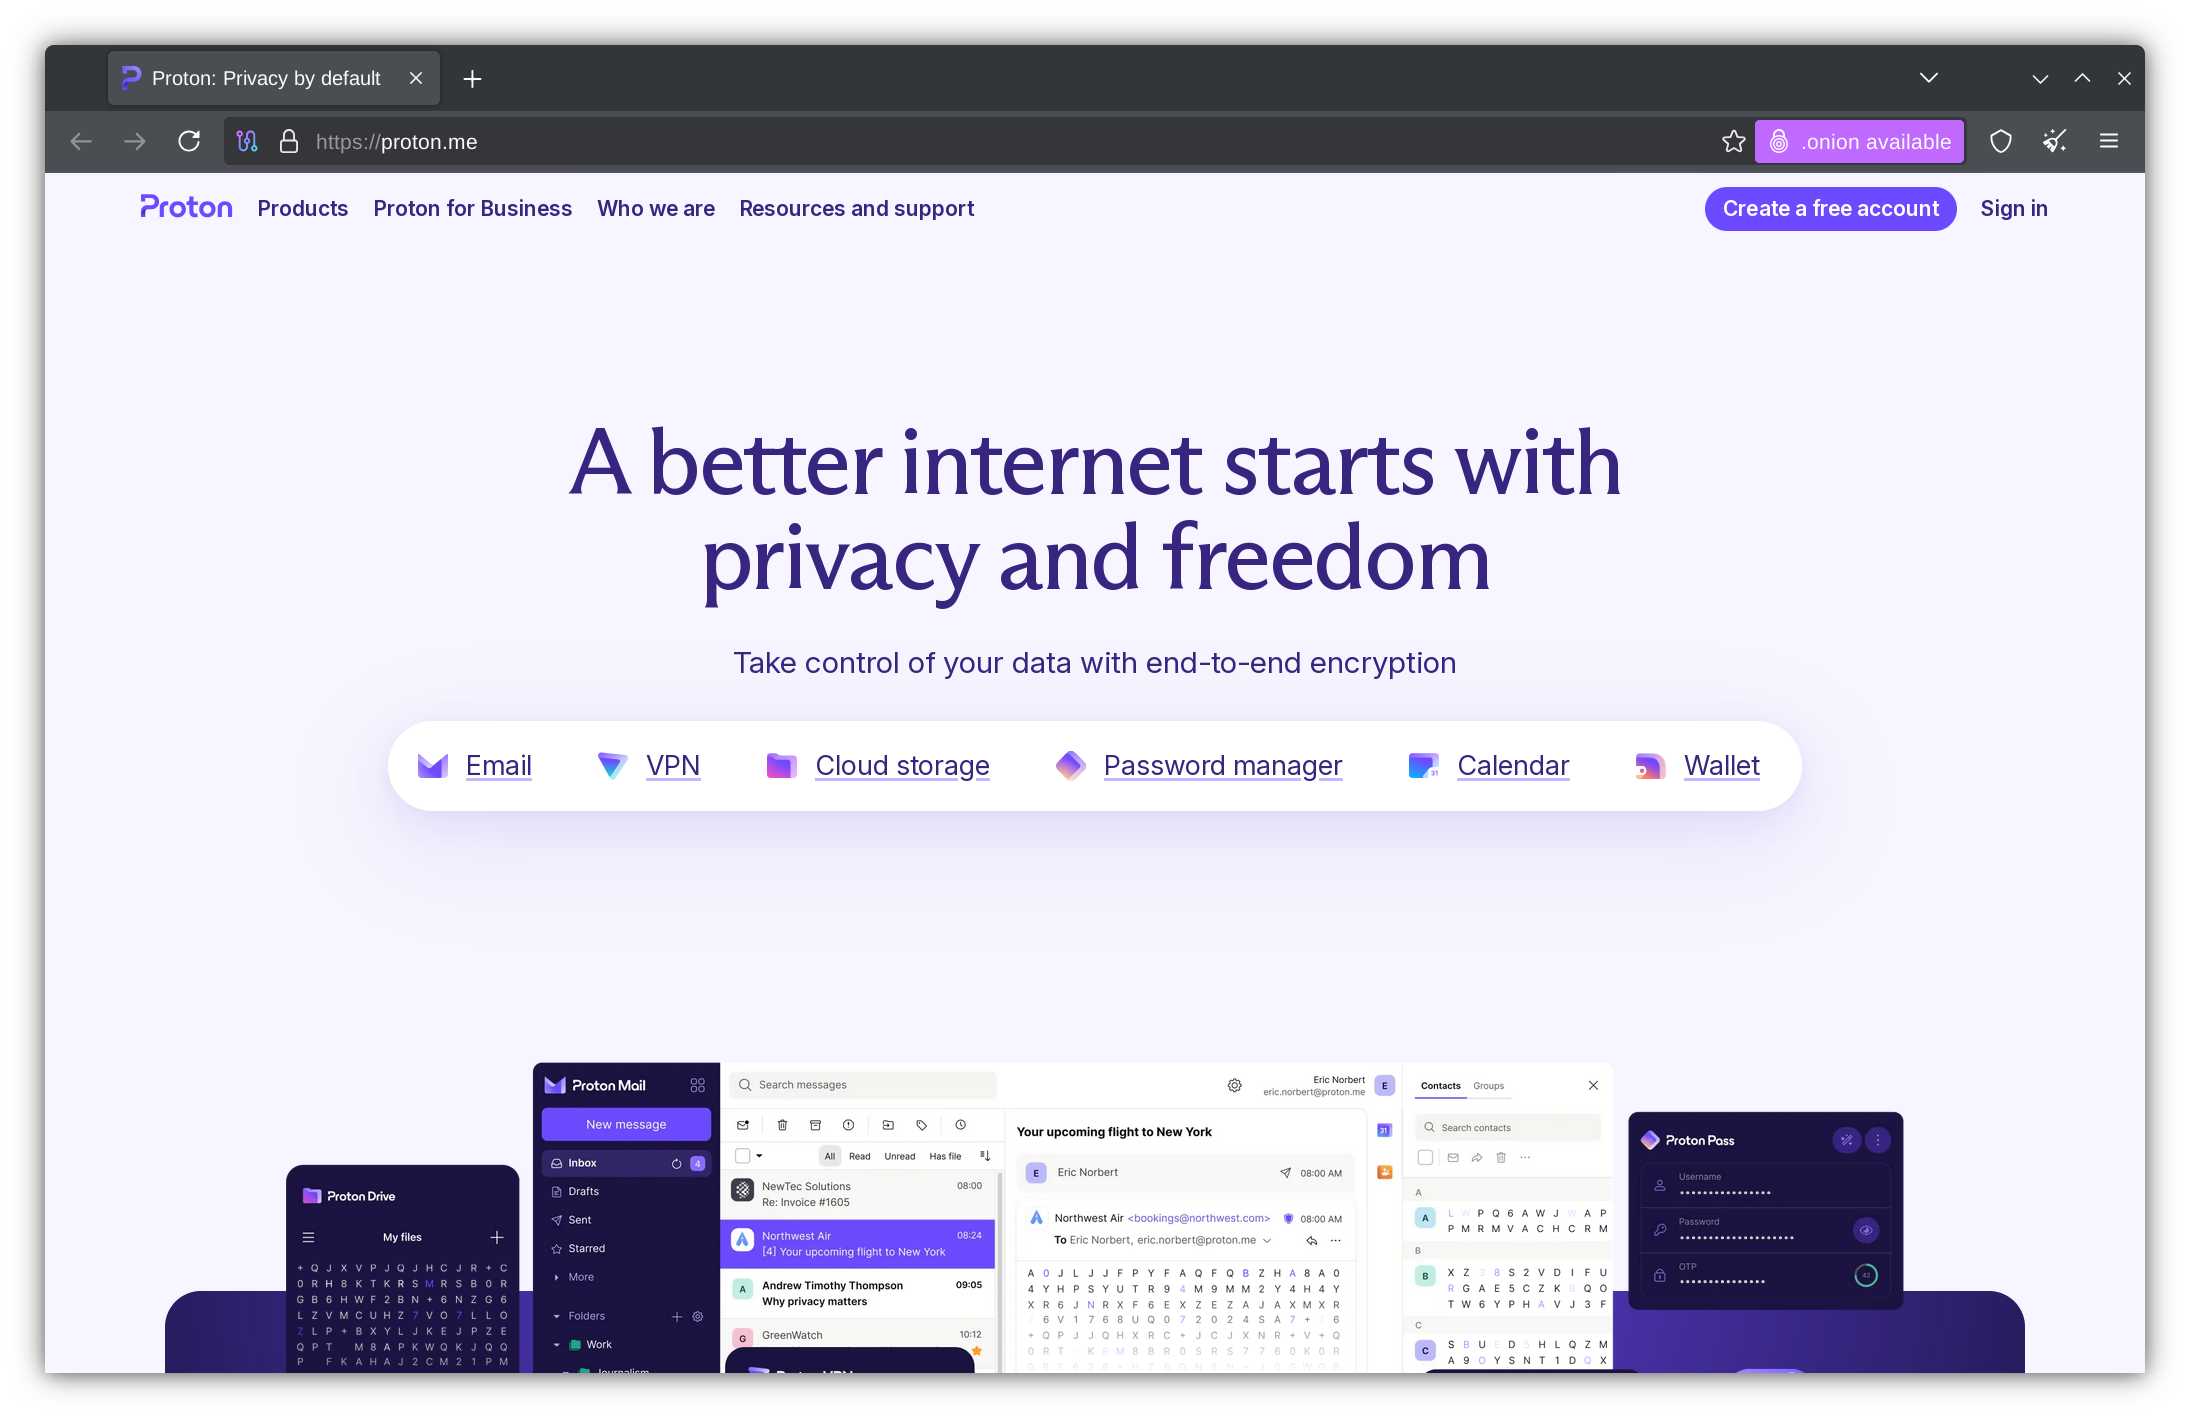
\includegraphics[width=\textwidth]{proton.me-.onion-popup.png}
    \caption{Botón \texttt{.onion} disponible}
\end{figure}

\begin{figure}[H]
    \centering
    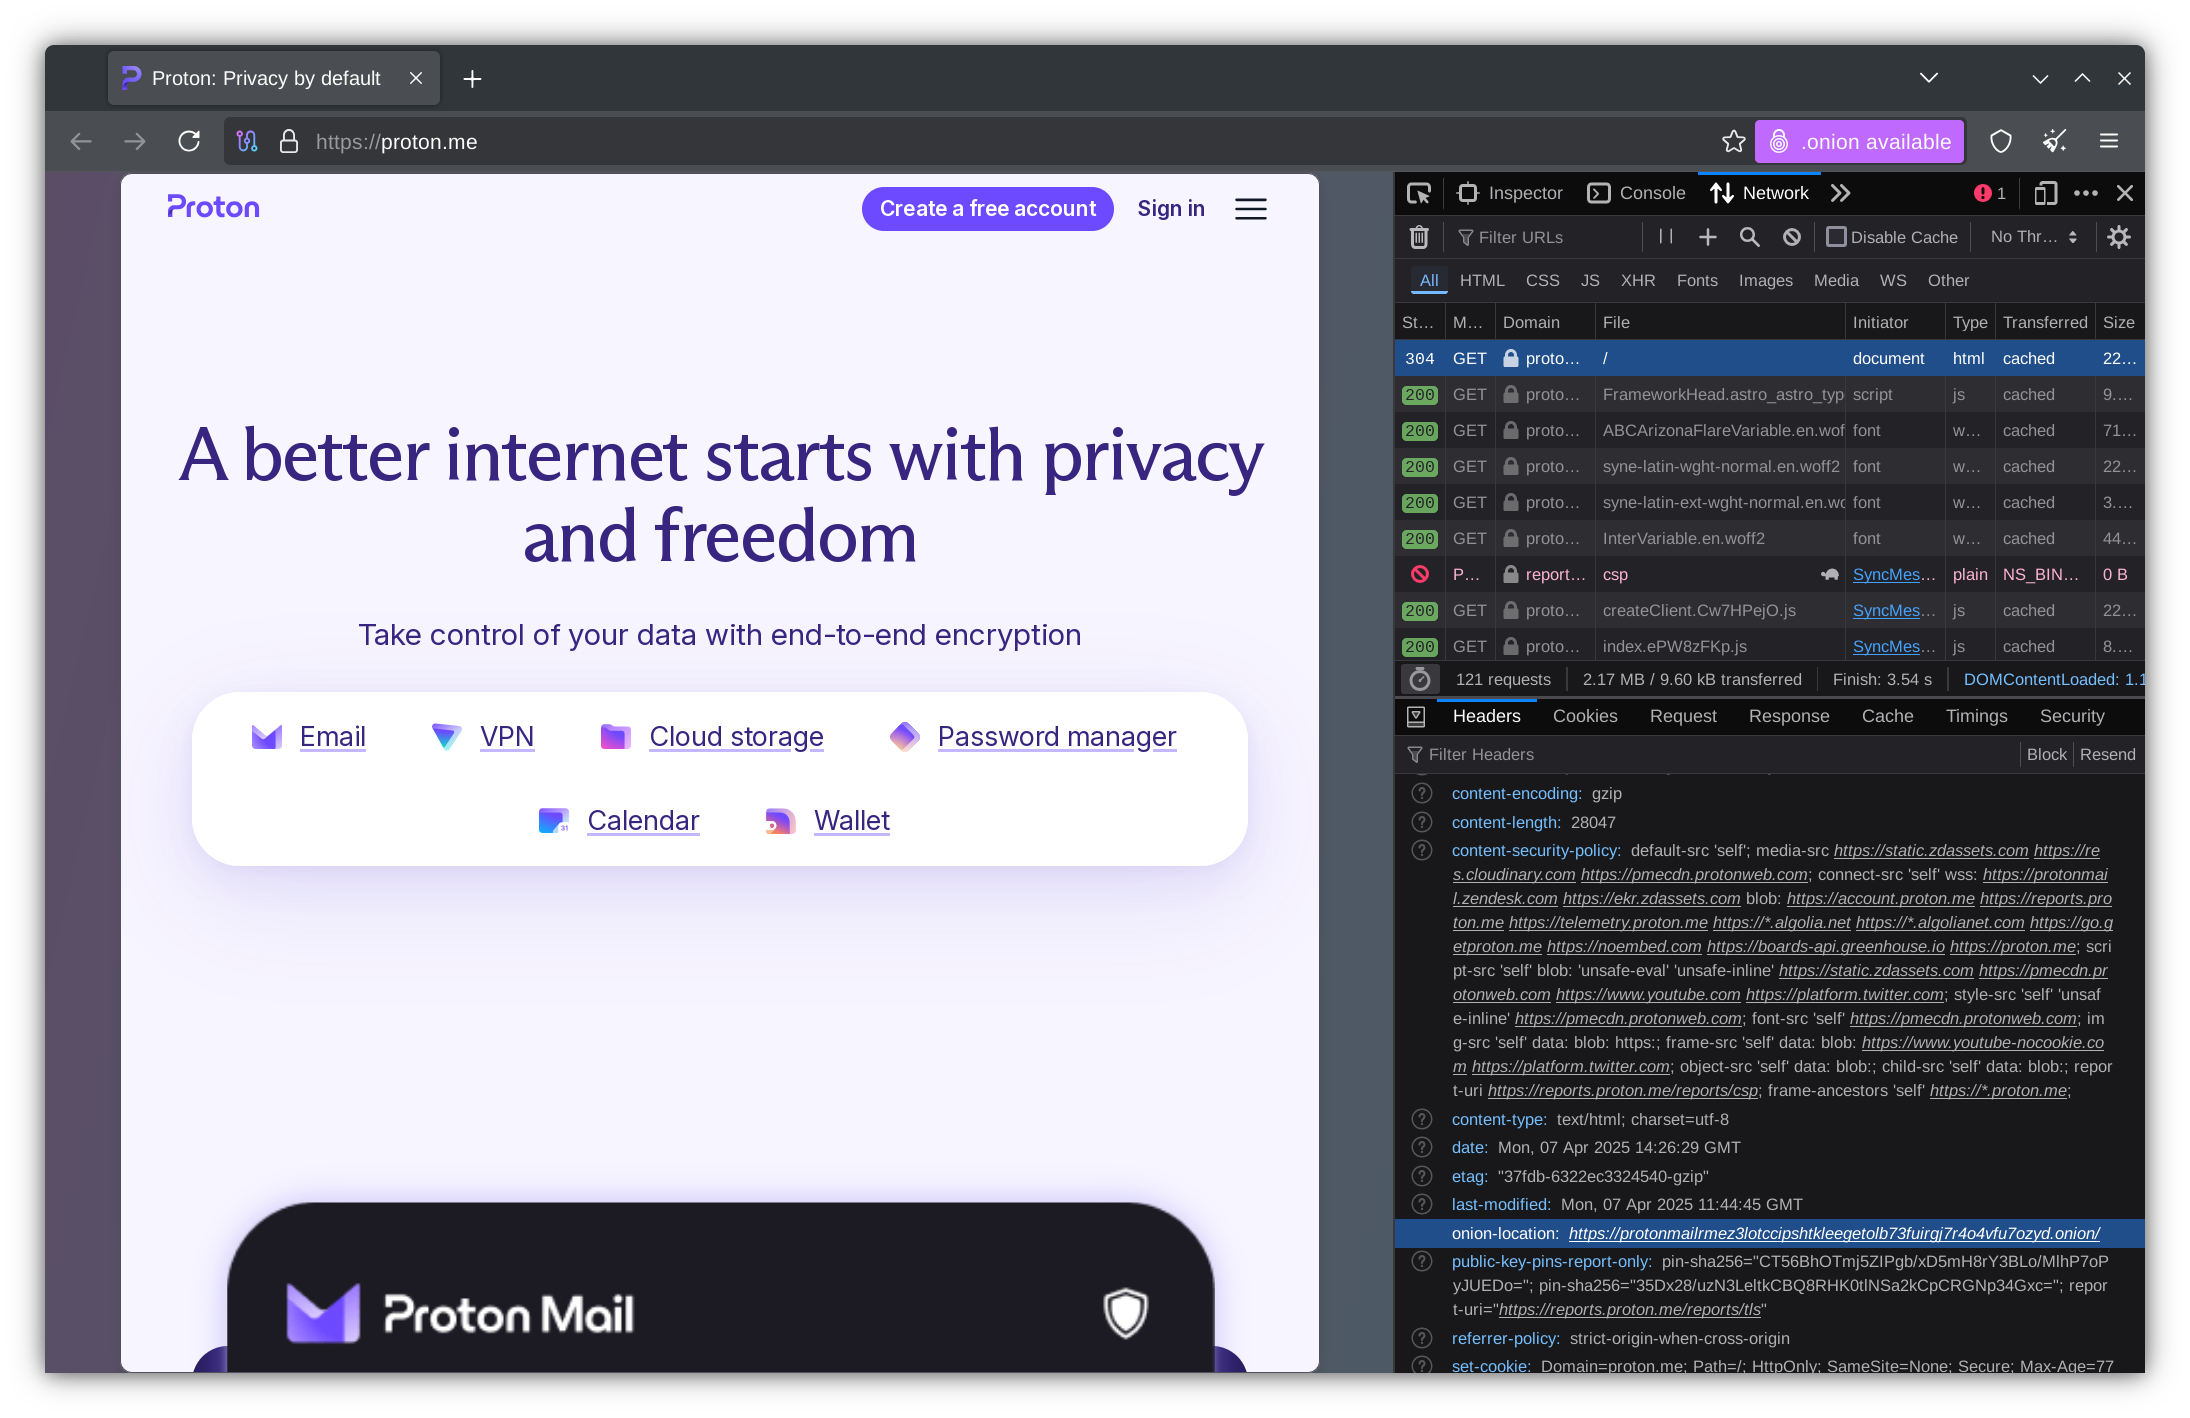
\includegraphics[width=\textwidth]{proton.me-onion-header.png}
    \caption{Detalle de la cabecera \texttt{Onion-Location} en \url{proton.me}}
\end{figure}

\subsubsection{Wikipedia en la red TOR}

Para encontrar la dirección \texttt{.onion} de Wikipedia utilizamos el motor de búsqueda Onion Search Engine que utilizamos para realizar una búsqueda tal y como haríamos en Google u otro buscador:

\begin{figure}[H]
    \centering
    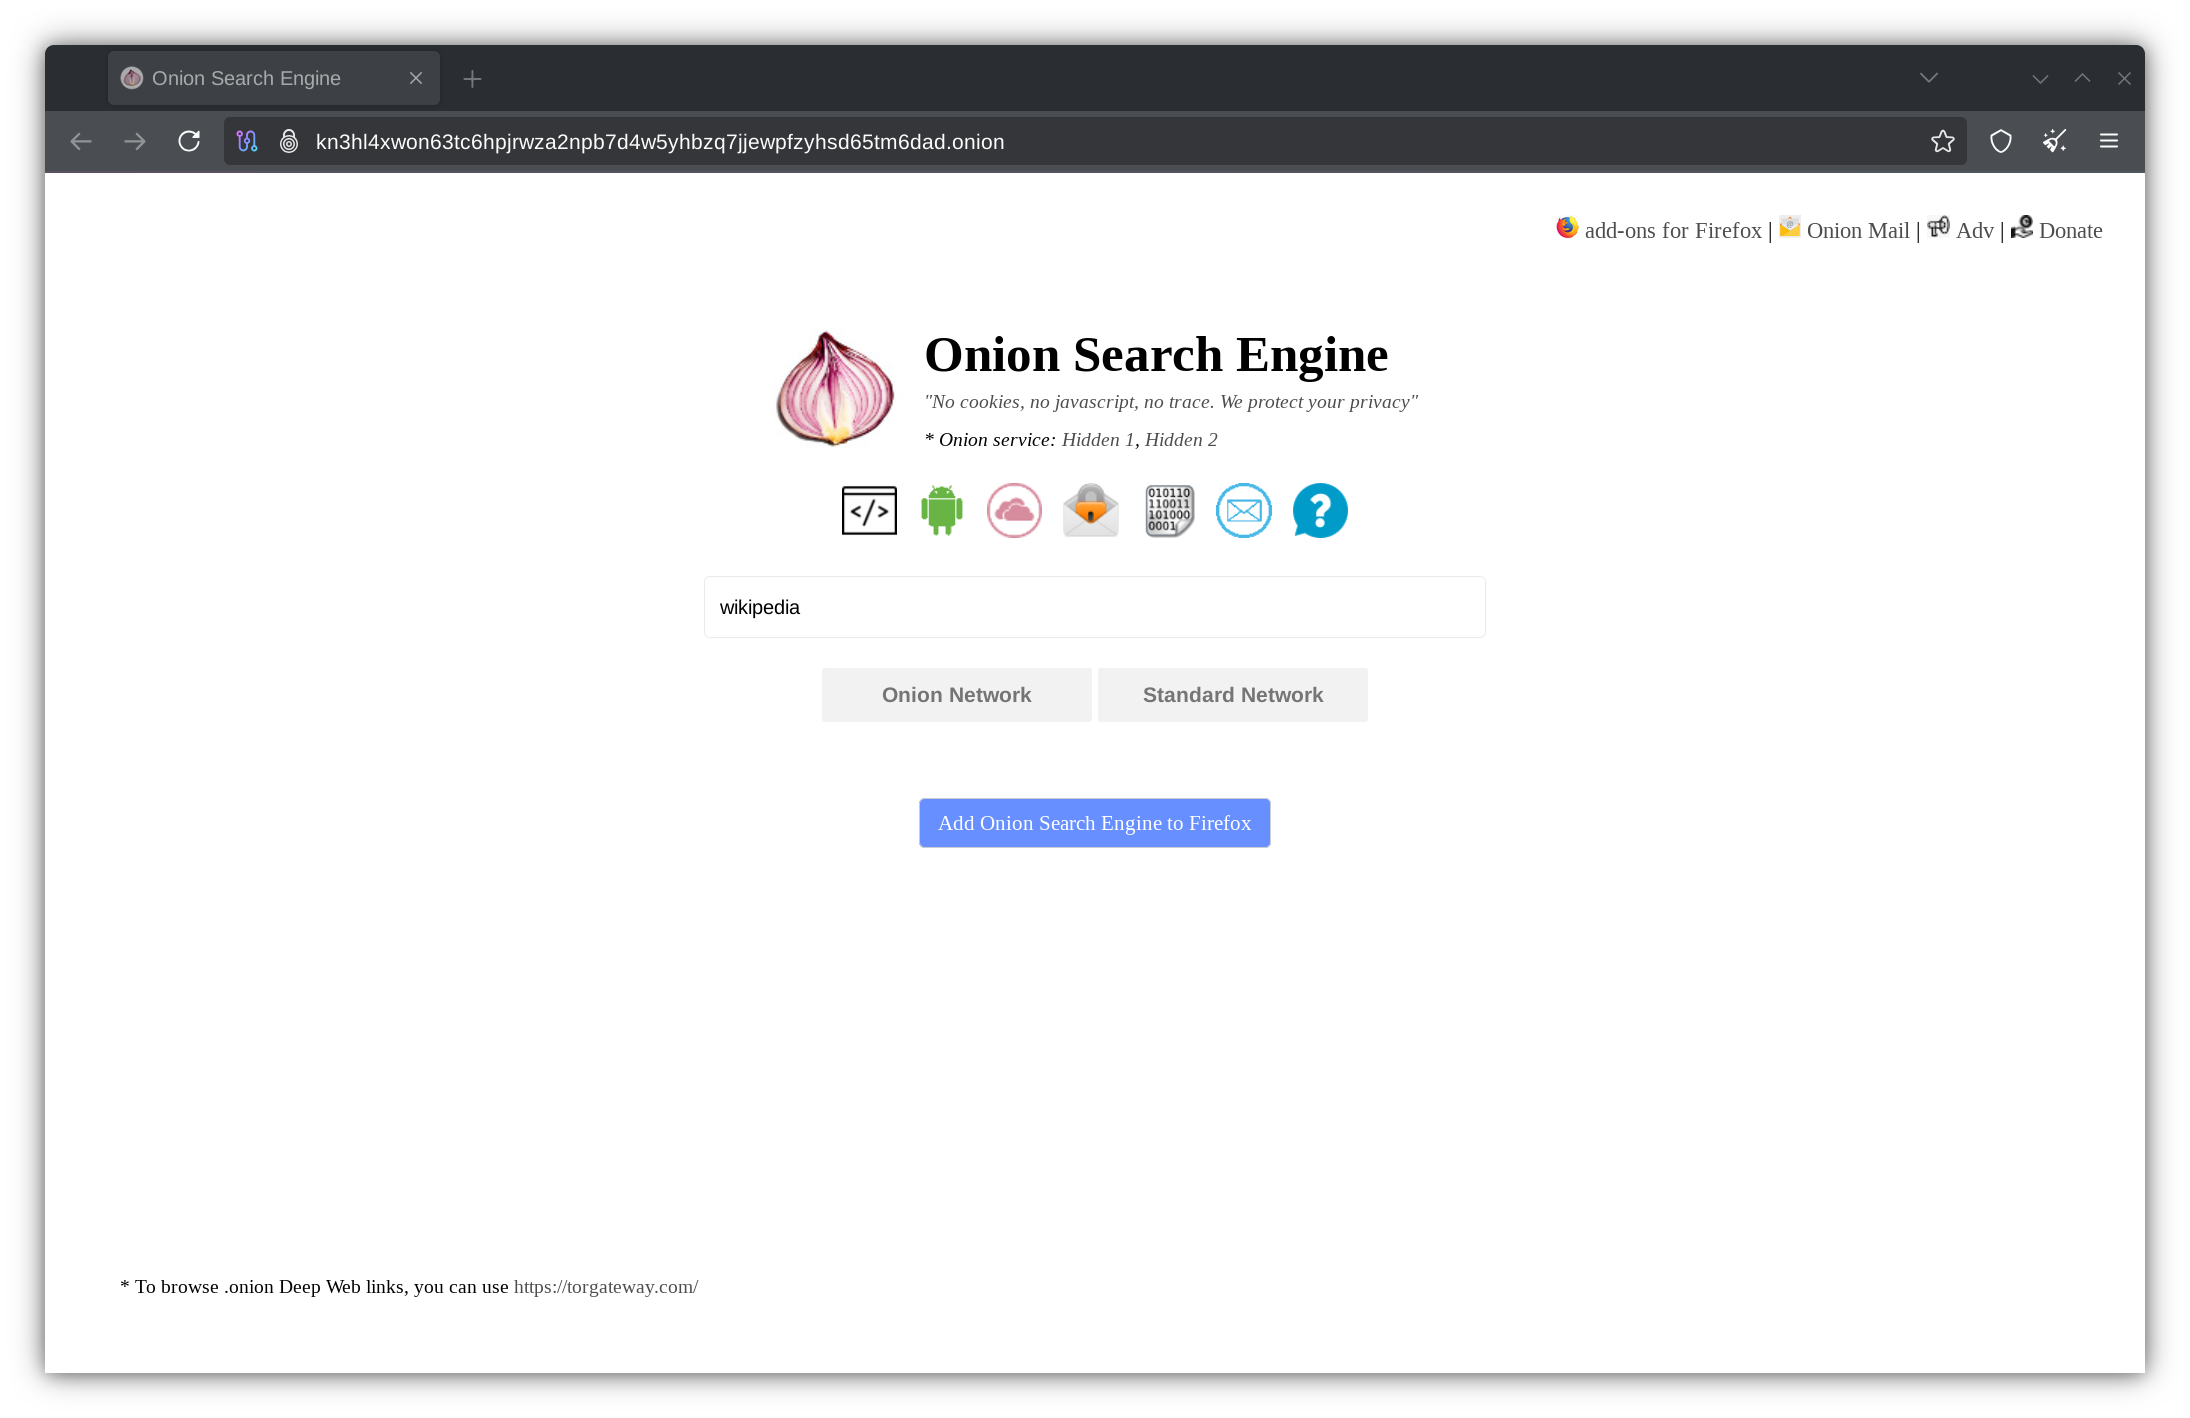
\includegraphics[width=\textwidth]{tor-onionengine.png}
    \caption{Motor de búsqueda Onion Search Engine}
\end{figure}

\begin{figure}[H]
    \centering
    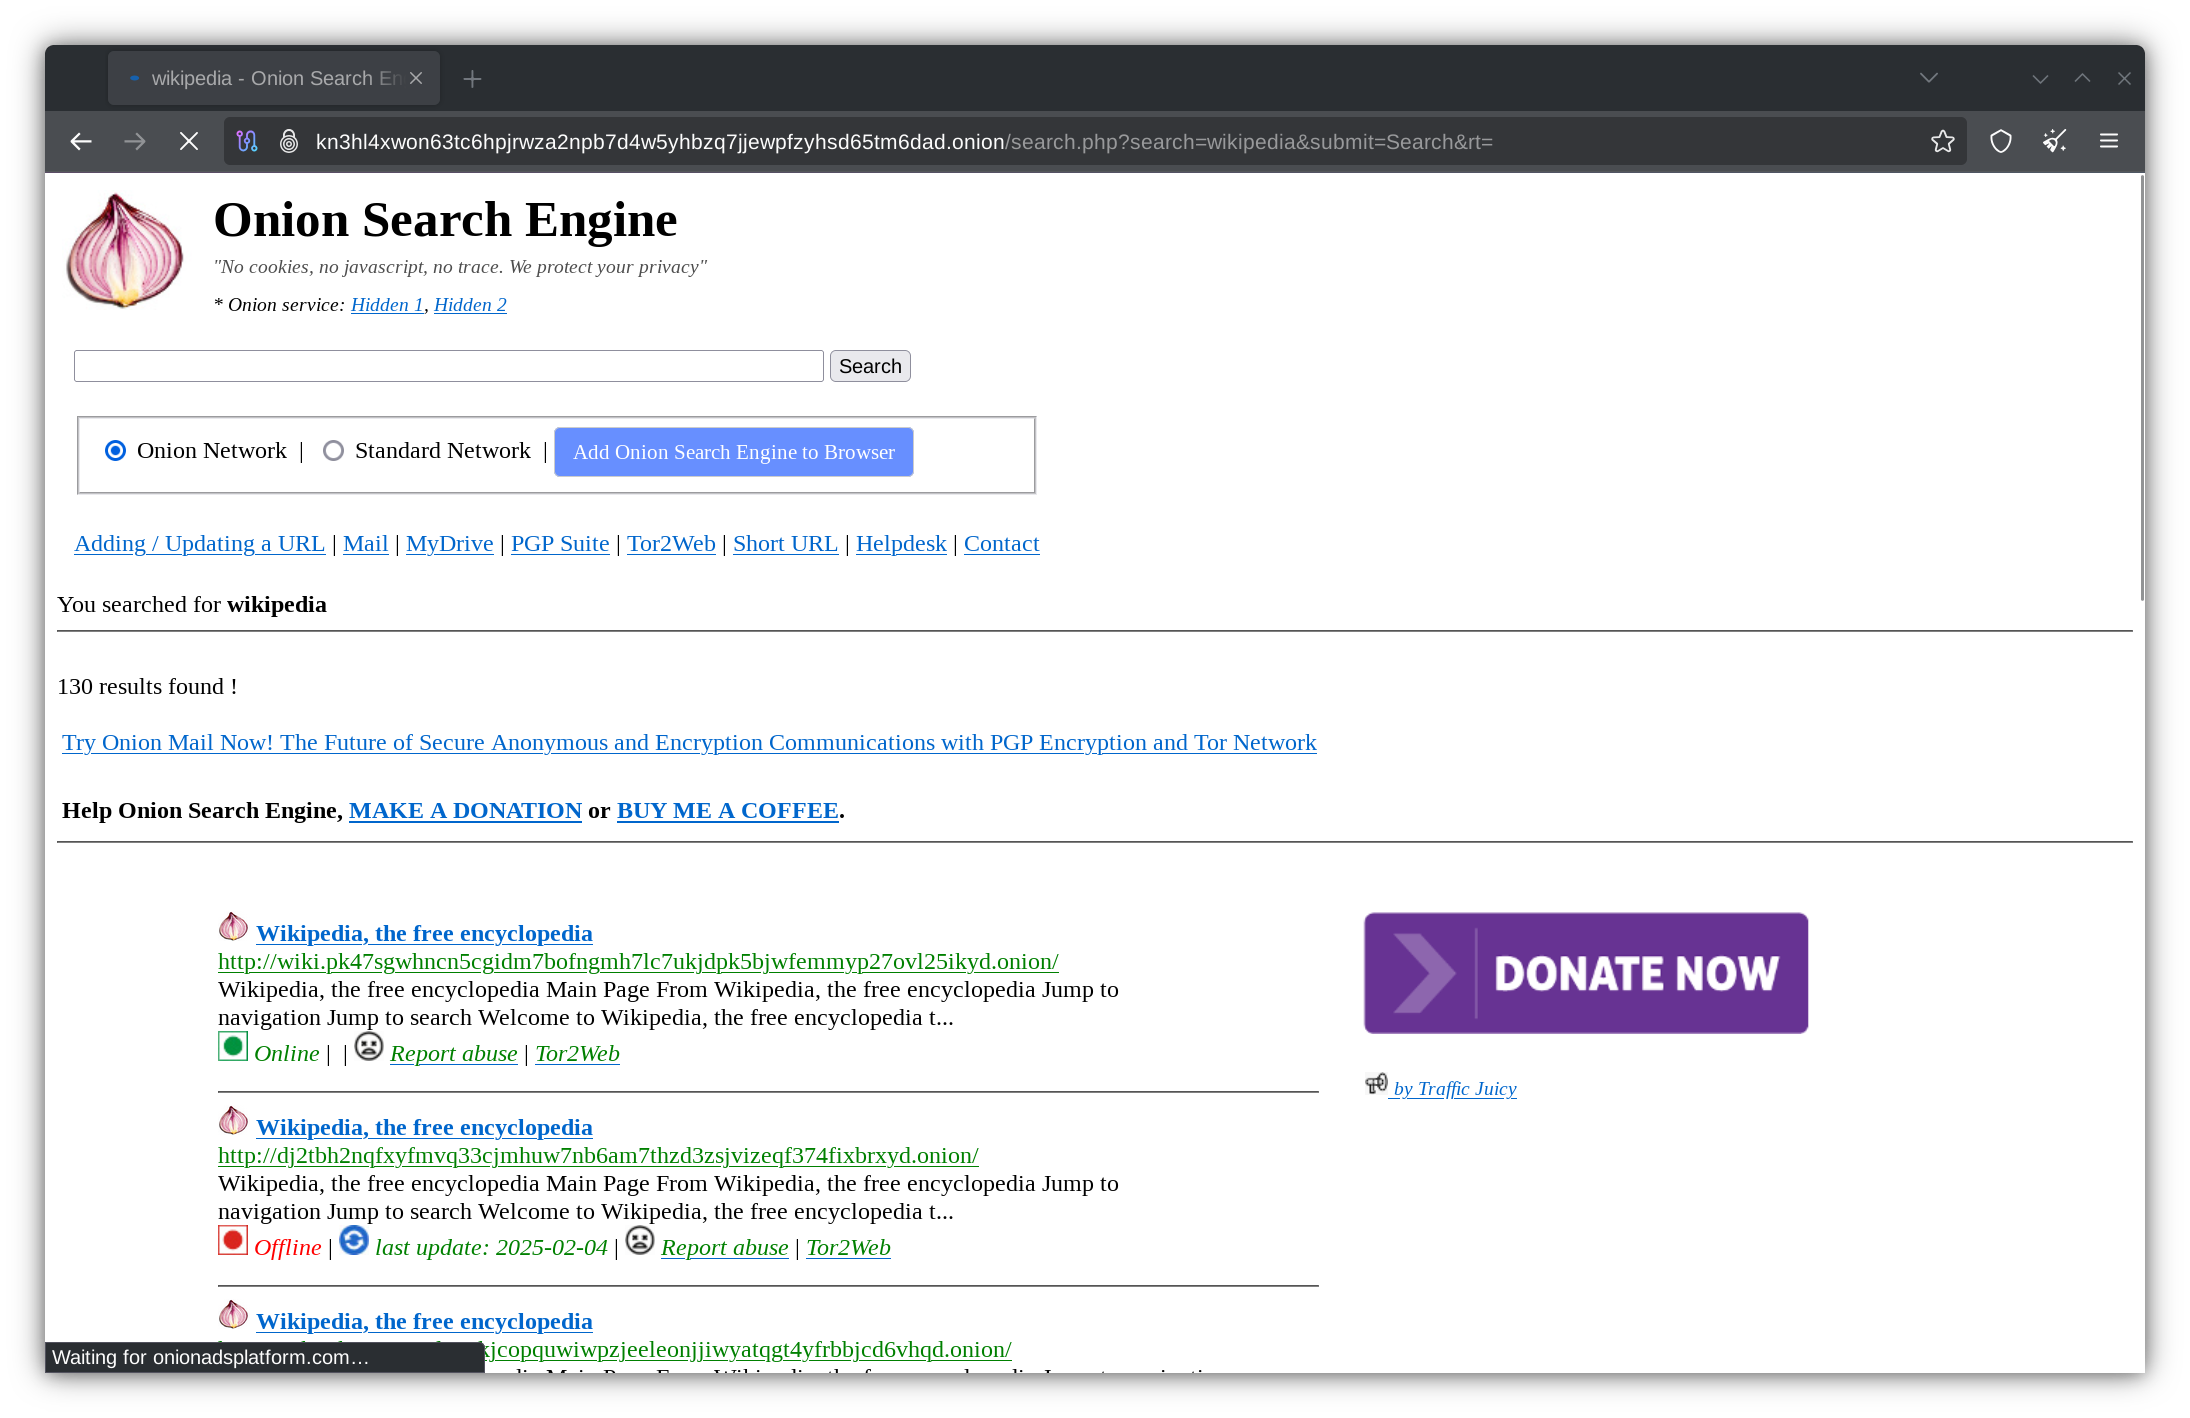
\includegraphics[width=\textwidth]{tor-onionengine-results.png}
    \caption{Resultados de la búsqueda en Onion Search Engine}
\end{figure}

Podemos comprobar que la versión de wikipedia en la red onion es idéntica a su versión en HTTP

\begin{figure}[H]
    \centering
    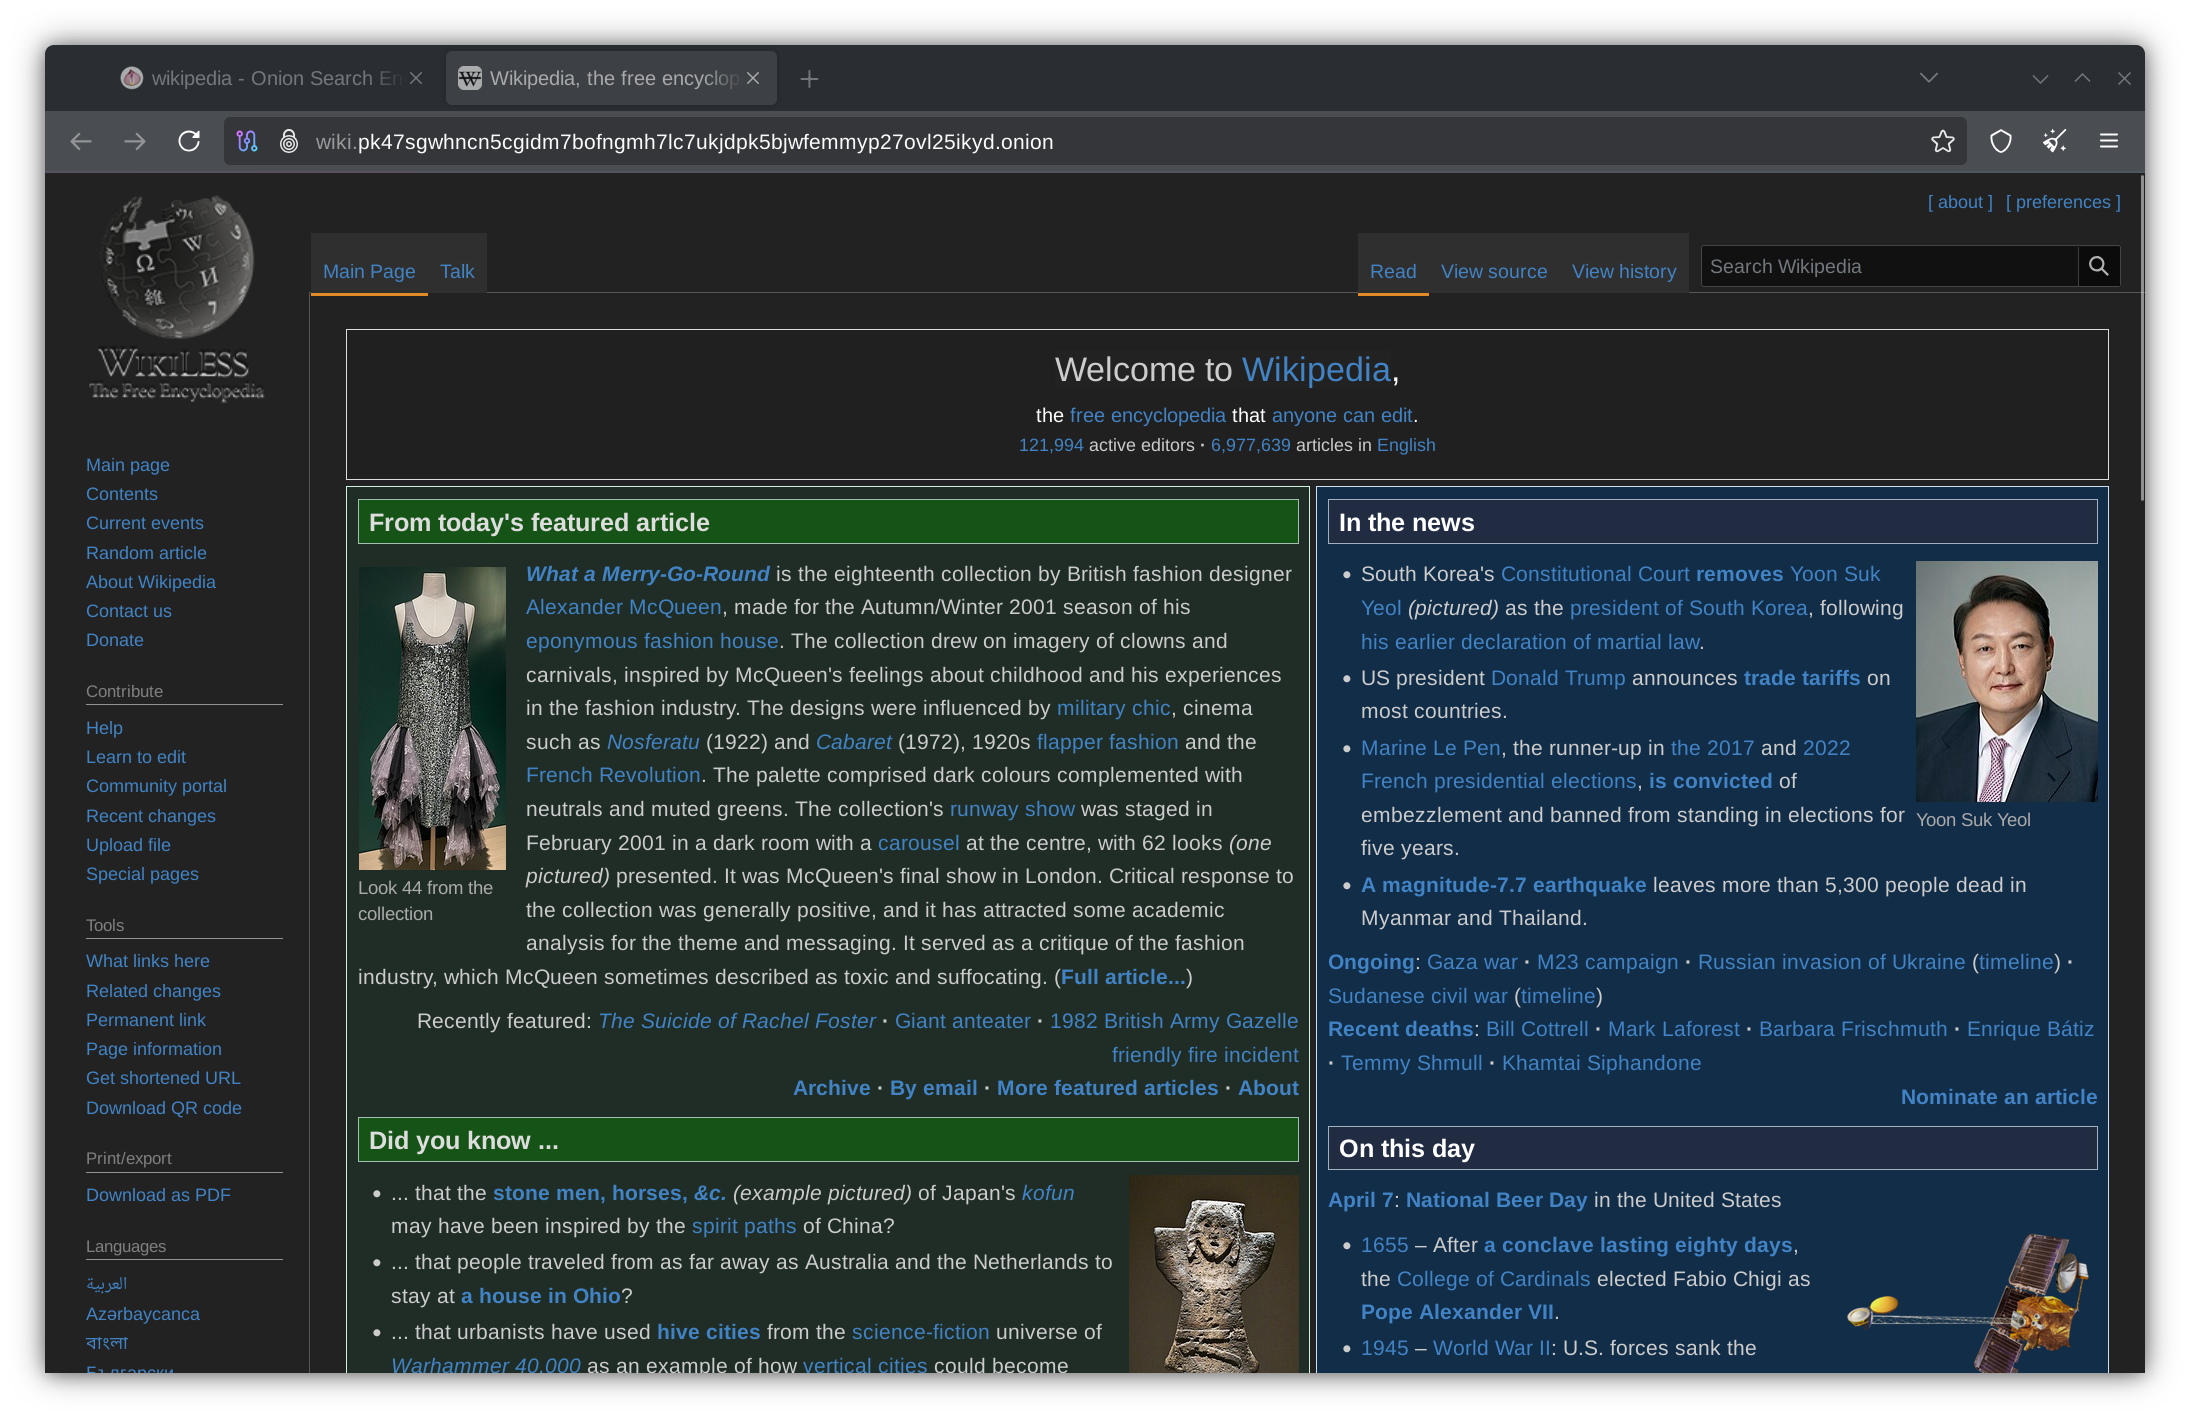
\includegraphics[width=\textwidth]{tor-wikipedia.png}
    \caption{Versión de Wikipedia en la red Onion}
\end{figure}